%% -*- ispell-local-dictionary: "british" -*-
%% Emilio Torres Manzanera
%% University of Oviedo
%% Time-stamp: <2014-03-05 mié 06:57 emilio on emilio-Satellite-P100>
%% =====================================================================
% \VignetteIndexEntry{Graphs in XKCD style}
% \VignettePackage{picante}
\documentclass[10pt]{article}
\usepackage[top=2in, bottom=1.5in, left=1in, right=1in]{geometry}
\usepackage{graphicx}
\usepackage{url}
\usepackage{hyperref}
\usepackage[utf8]{inputenc}     % Linux
% \usepackage[activeacute,spanish]{babel} % Spanishs titles
% \usepackage{fouriernc}          % Type of font
\usepackage[T1]{fontenc} 
\usepackage{fancybox,fancyvrb,calc} % first, fancybox, and then, fancyvrb
\usepackage{Sweave}% After fancybox!!!
%\SweaveOpts{eval=FALSE}
\DefineVerbatimEnvironment{Sinput}{Verbatim}{fontshape=sl, xleftmargin=-3em, fontsize=\small,gobble=2,numbers=left}
\DefineVerbatimEnvironment{Soutput}{Verbatim}{xleftmargin=-2.5em, fontsize=\small,formatcom=\color{azulpautipografia},numbers=left,stepnumber=3}

% See 
% Customizing Sweave to Produce A Better Looking LaTEX Output
% Ross Ihaka
% \DefineVerbatimEnvironment{Sinput}{Verbatim} {xleftmargin=2em}
% \DefineVerbatimEnvironment{Soutput}{Verbatim}{xleftmargin=2em}
% \DefineVerbatimEnvironment{Scode}{Verbatim}{xleftmargin=2em}
% \fvset{listparameters={\setlength{\topsep}{0pt}}}
% \renewenvironment{Schunk}{\vspace{\topsep}}{\vspace{\topsep}}


\title{An introduction to the xkcd package}
\author{Emilio Torres-Manzanera\\ (torres@uniovi.es)}
\date{March 2014}

\begin{document}


 % Pdf images must embed the fonts. 


\setkeys{Gin}{width=0.5\textwidth} % After begin{document}


\maketitle

\begin{abstract}
    
    \end{abstract}

\begin{center}
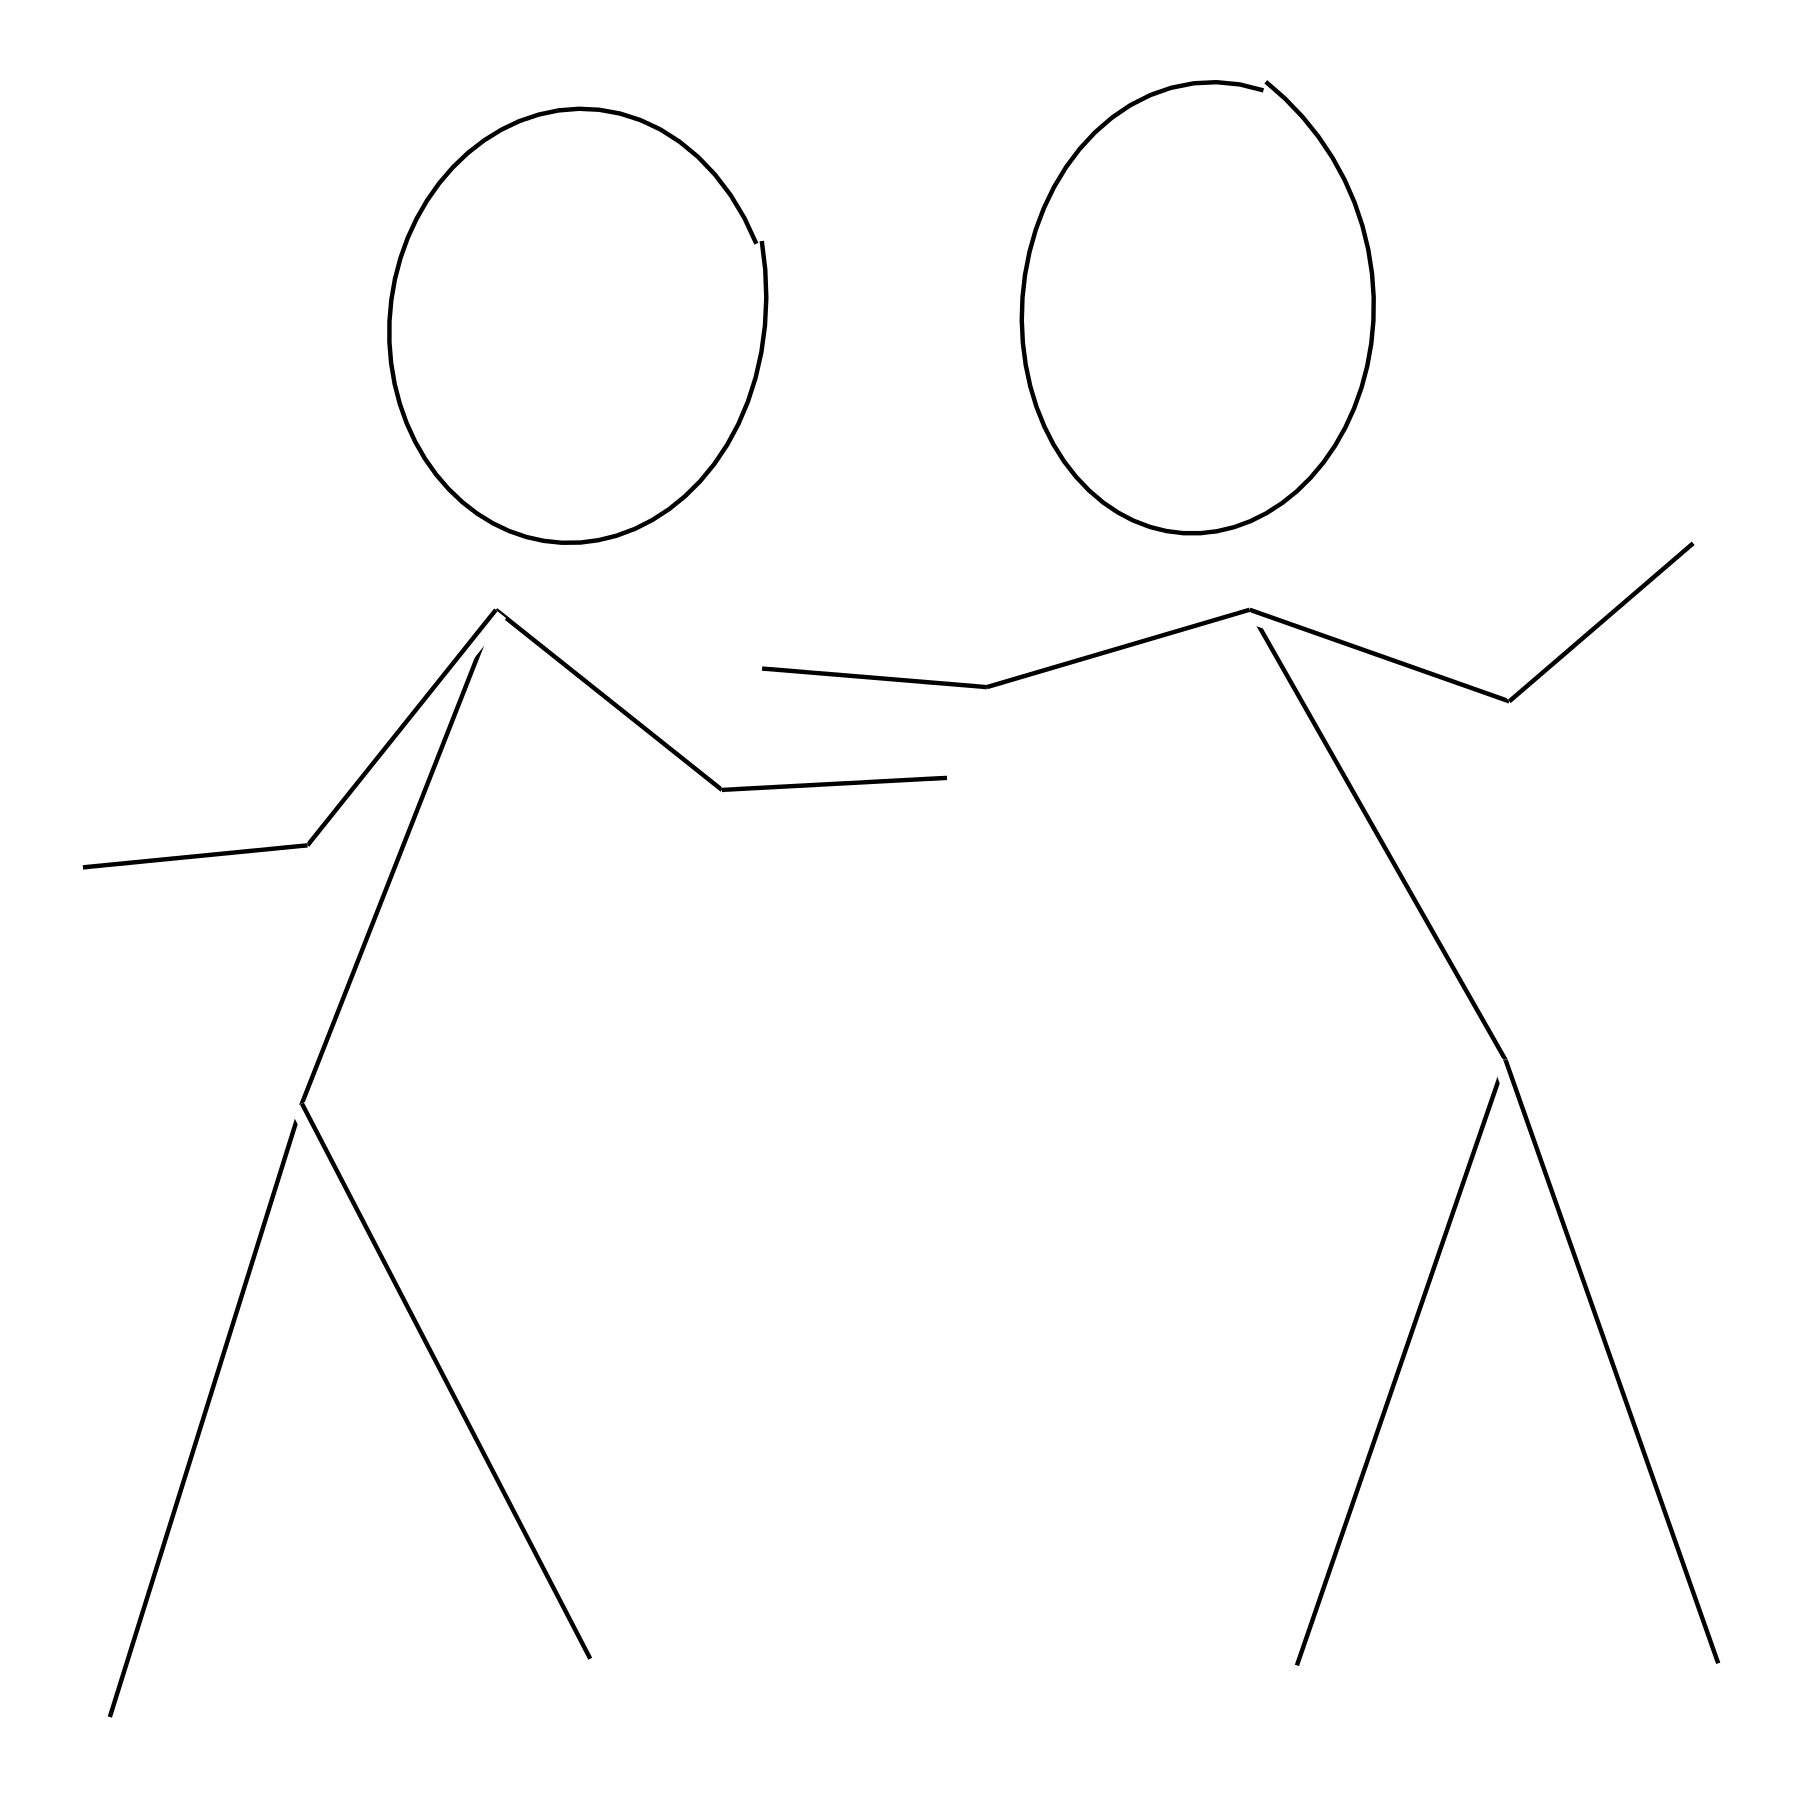
\includegraphics{xkcd-intro-twoman}

\end{center}
\tableofcontents

\bigskip
\section{Graph Gallery}

See more examples at \url{http://xkcd.r-forge.r-project.org/}.

\section{The XKCD fonts}

The package \texttt{xkcd} uses the XKCD fonts. Therefore, an easy way to check whether this fonts are installed in the computer is typing the following code and comparing the graphs:


\begin{center}
\begin{Schunk}
\begin{Sinput}
> library(sysfonts)
> library(ggplot2)
> if( "xkcd.ttf" %in% font.files()) {
+   font.add("xkcd",  regular = "xkcd.ttf")
+   p <-  ggplot() + geom_point(aes(x=mpg, y=wt), data=mtcars) + 
+     theme(text = element_text(size = 16, family = "xkcd"))
+ } else  {
+   warning("Not xkcd fonts installed!")
+   p <-  ggplot() + geom_point(aes(x=mpg, y=wt), data=mtcars) 
+ }
> p
\end{Sinput}
\end{Schunk}
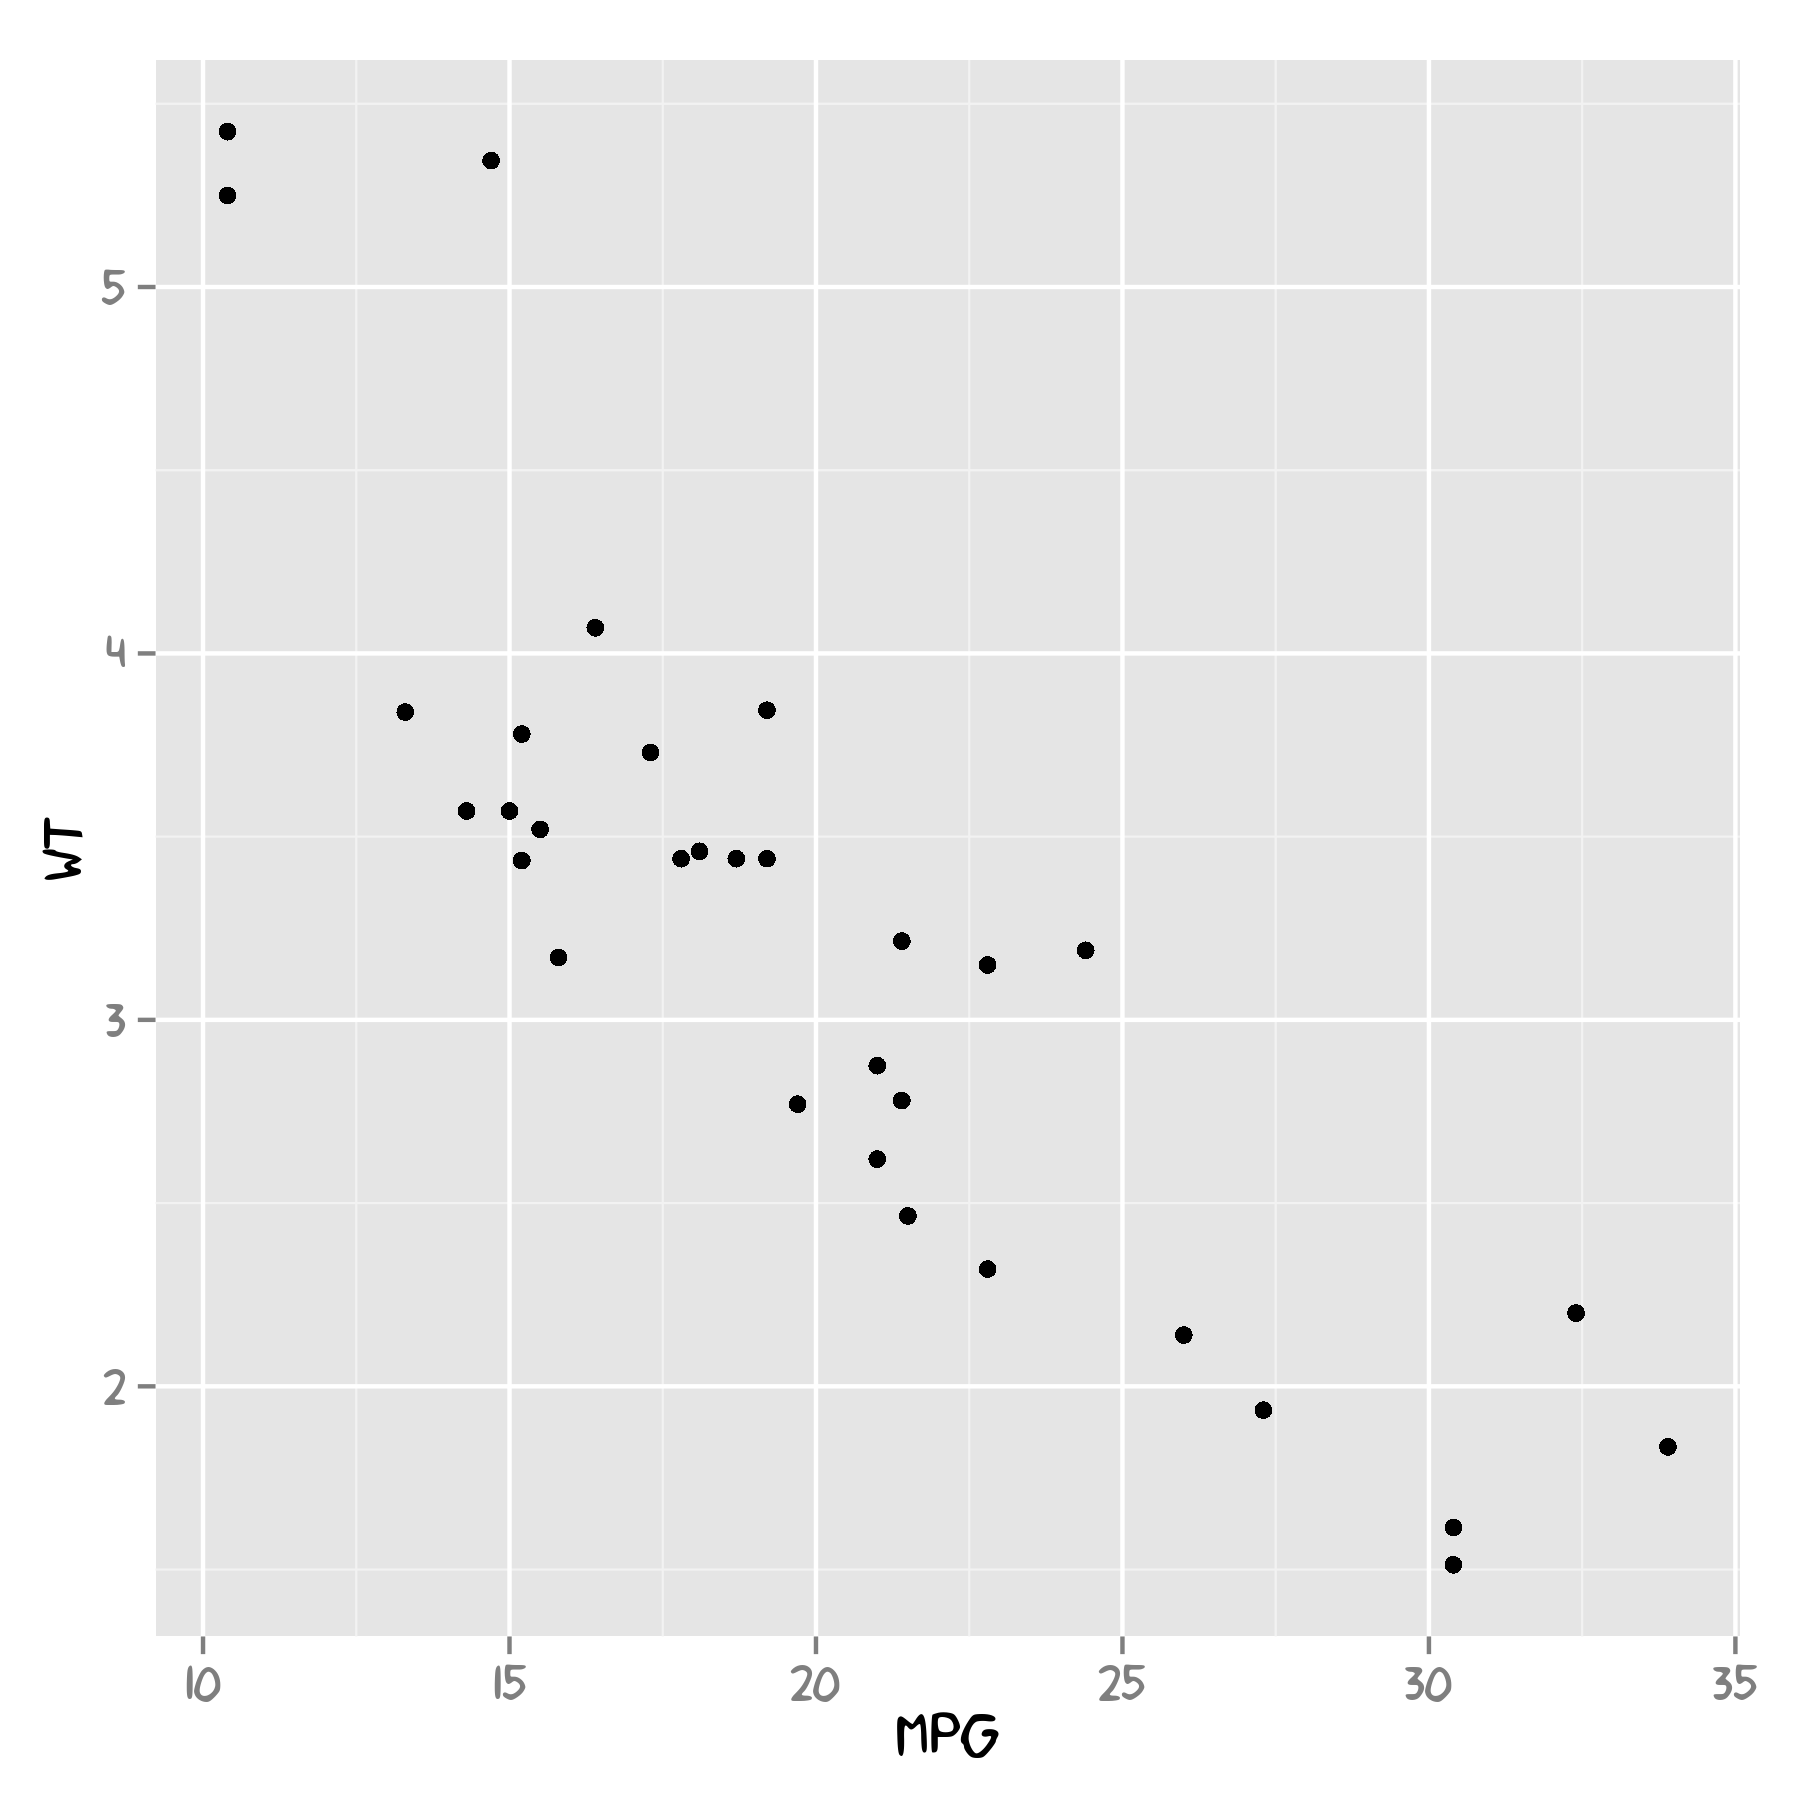
\includegraphics{xkcd-intro-003}
\end{center}

\subsection{Installing fonts in R}



The XKCD fonts are not installed in the system. You can use the package \texttt{sysfonts}, and the function \texttt{font.paths()} to check the current search path or add a new one, and use \texttt{font.files()} to list available font files in the search path.

\begin{Schunk}
\begin{Sinput}
> library(sysfonts)
> download.file("http://simonsoftware.se/other/xkcd.ttf", dest="xkcd.ttf", mode="wb")
> font.paths()
> system("mkdir ~/.fonts")
> system("cp xkcd.tff -t ~/.fonts")
> font.files()
> font.add("xkcd",  regular = "xkcd.ttf")
> font.families()
\end{Sinput}
\end{Schunk}



\subsection{Saving the graphs}

\subsubsection{png}

\begin{Schunk}
\begin{Sinput}
> font.add("xkcd",  regular = "xkcd.ttf")
> p <-  ggplot() + geom_point(aes(x=mpg, y=wt), data=mtcars) + 
+   theme(text = element_text(size = 16, family = "xkcd"))
> ggsave("fig.png", p)
\end{Sinput}
\end{Schunk}

\subsubsection{pdf}
Yixuan Qiu, author of the packages \texttt{sysfonts} and \texttt{showtext}, provides an example of saving pdf plots:

\begin{Schunk}
\begin{Sinput}
> library(showtext)
> font.add("xkcd", "xkcd.ttf")
> pdf("showtext.pdf")
> showtext.begin()
> print(p)
> showtext.end()
> dev.off()
\end{Sinput}
\end{Schunk}




\section{Installing xkcd}

The xkcd homepage is located at \url{http://xkcd.r-forge.r-project.org}. 
From within R, you can install the latest version of xkcd by typing 
\begin{Schunk}
\begin{Sinput}
> install.packages("xkcd",dependencies = TRUE)
\end{Sinput}
\end{Schunk}

Then, you may want to see the vignette and check the code:
\begin{Schunk}
\begin{Sinput}
> help(package="xkcd")
> vignette("xkcd-intro") # it opens the pdf
> browseVignettes(package = "xkcd") # To browse the pdf, R and Rnw
\end{Sinput}
\end{Schunk}

Once the package has been installed, it can be loaded by typing:

\begin{Schunk}
\begin{Sinput}
> library(xkcd)
\end{Sinput}
\end{Schunk}


\section{Axis}




\begin{center}
    Man: No, I just think I can do better than someone who doesn't label her axes. Title text: And if you labeled your axes, I could tell you exactly how MUCH better.  {\tiny
    \url{http://xkcd.com/833/}
    \url{http://imgs.xkcd.com/comics/convincing.png}}
    
    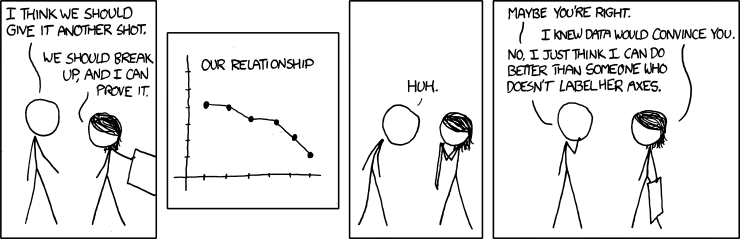
\includegraphics[width=0.7\textwidth]{convincing}

   
\end{center}






\begin{center}
\begin{Schunk}
\begin{Sinput}
> xrange <- range(mtcars$mpg)
> yrange <- range(mtcars$wt)
> set.seed(123) # for reproducibility
> p <- ggplot() + geom_point(aes(mpg, wt), data=mtcars) + 
+   xkcdaxis(xrange,yrange)
> p
\end{Sinput}
\end{Schunk}
\includegraphics{xkcd-intro-010}
\end{center}



\section{Cartoon characters}

To include cartoon characters in the graph, use the \texttt{xkcdman} function.

\begin{center}
\begin{Schunk}
\begin{Sinput}
> ratioxy <- diff(xrange)/diff(yrange)
> mapping <- aes(x,  y,
+                scale,
+                ratioxy,
+                angleofspine ,
+                anglerighthumerus,
+                anglelefthumerus,
+                anglerightradius,
+                angleleftradius,
+                anglerightleg,
+                angleleftleg,
+                angleofneck,
+                linetype=city)
> dataman <- data.frame(x= c(15,30), y=c(3, 4),
+                       scale = c(0.3,0.51) ,
+                       ratioxy = ratioxy,
+                       angleofspine =  -pi/2  ,
+                       anglerighthumerus = c(pi/4, -pi/6),
+                       anglelefthumerus = c(pi/2 + pi/4, pi +pi/6),
+                       anglerightradius = c(pi/3, -pi/3),
+                       angleleftradius = c(pi/3, -pi/3),
+                       anglerightleg = 3*pi/2  - pi / 12,
+                       angleleftleg = 3*pi/2  + pi / 12 ,
+                       angleofneck = runif(1, 3*pi/2-pi/10, 3*pi/2+pi/10),
+                       city=c("Liliput","Brobdingnag"))
> q <- ggplot() + geom_point(aes(mpg, wt, colour=as.character(vs)), data=mtcars) + 
+   xkcdaxis(xrange,yrange) + xkcdman(mapping, dataman)
> q
\end{Sinput}
\end{Schunk}
\includegraphics{xkcd-intro-011}
\end{center}

\subsection{Facets}

\begin{center}
\begin{Schunk}
\begin{Sinput}
> ggplot() + geom_point(aes(mpg, wt), data=mtcars) + 
+   xkcdaxis(xrange,yrange) + xkcdman(mapping, dataman) +
+   facet_grid(.~vs)
\end{Sinput}
\end{Schunk}
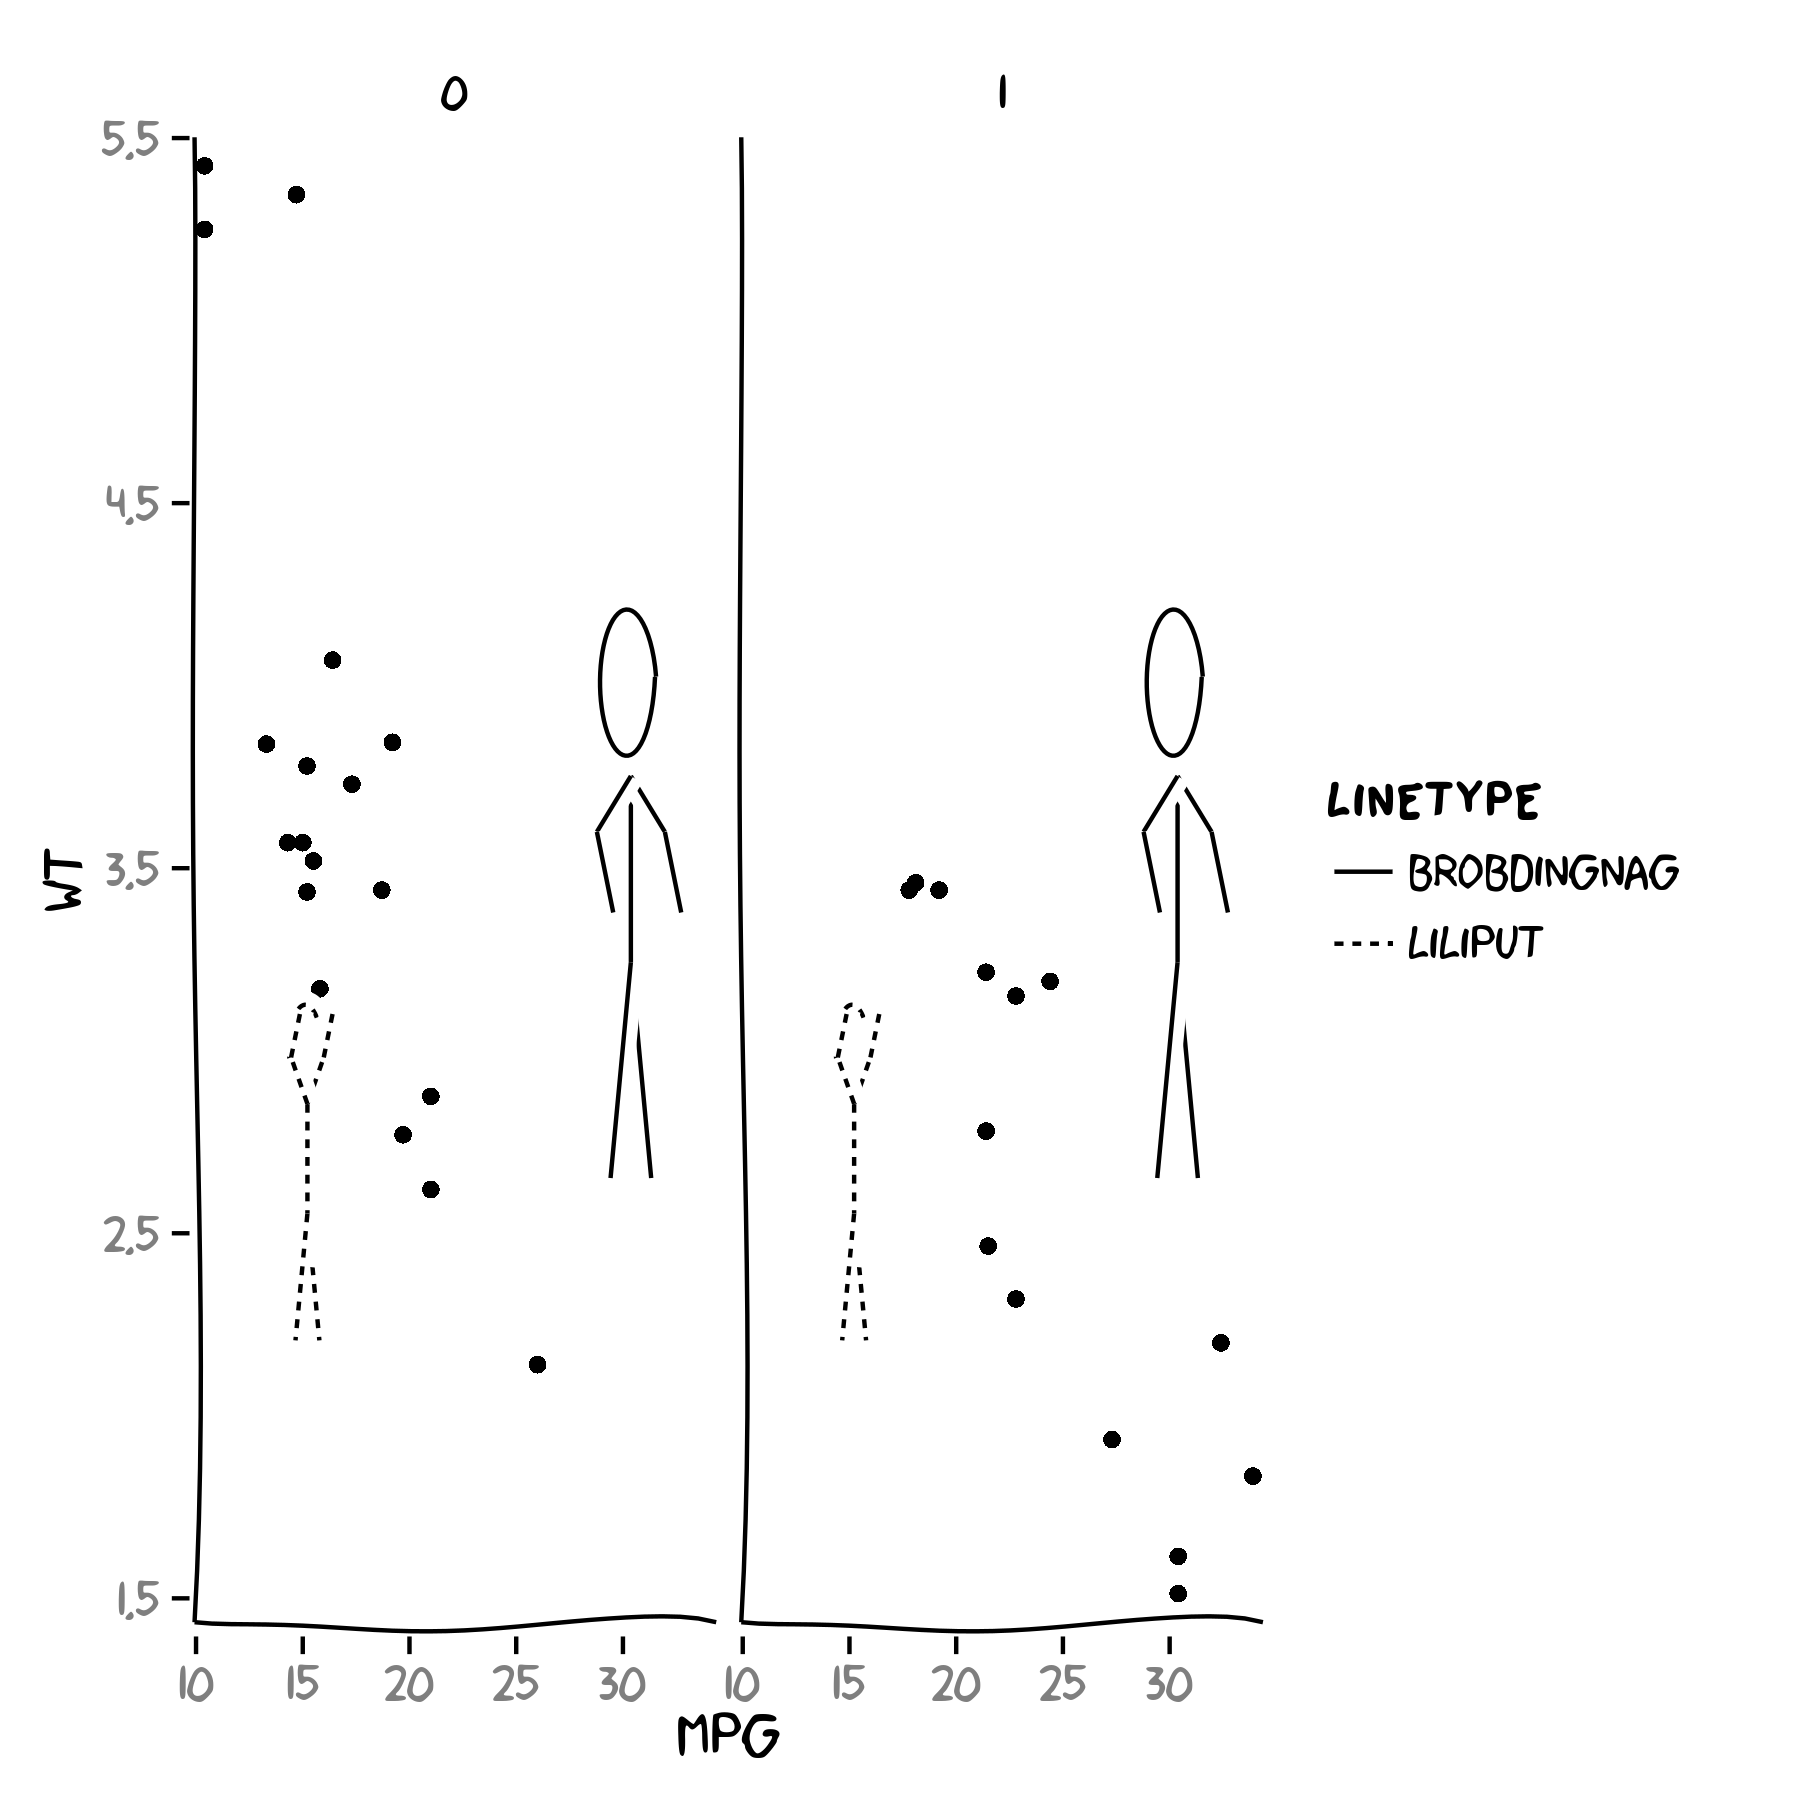
\includegraphics{xkcd-intro-facetvs}
\end{center}


\begin{center}
\begin{Schunk}
\begin{Sinput}
> ggplot() + geom_point(aes(mpg, wt), data=mtcars) + 
+   xkcdaxis(xrange,yrange) + xkcdman(mapping, dataman) +
+   facet_grid(.~city)
\end{Sinput}
\end{Schunk}
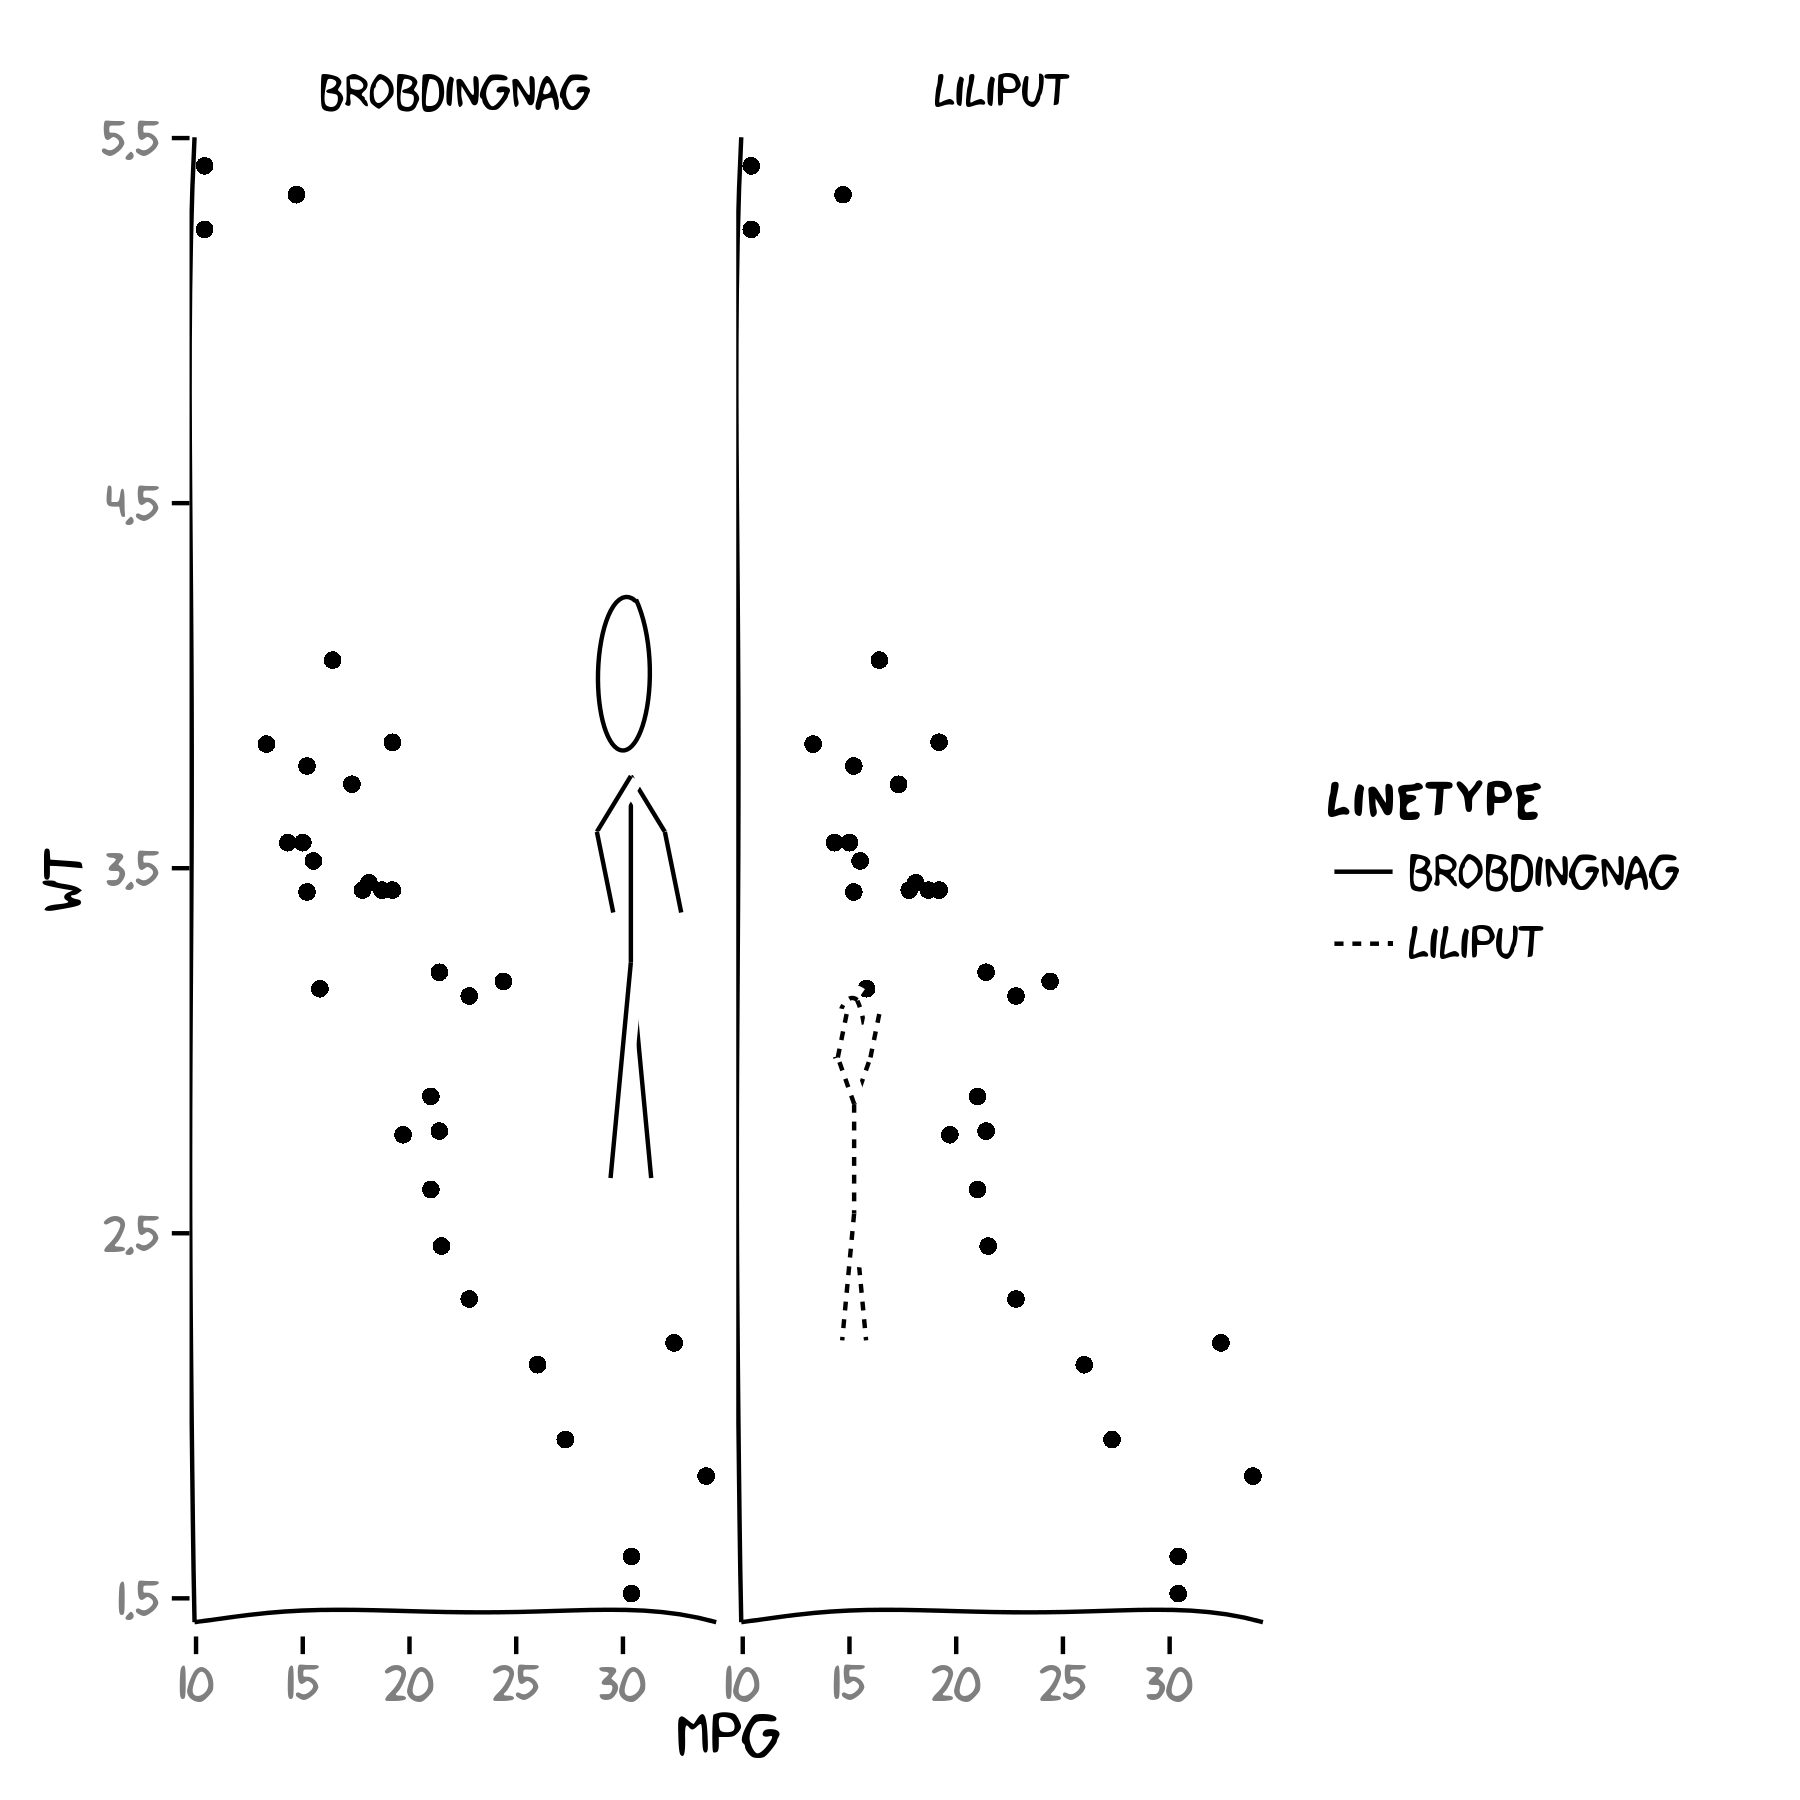
\includegraphics{xkcd-intro-facetcity}
\end{center}


\subsection{Angles of the xkcdman}

\begin{center}
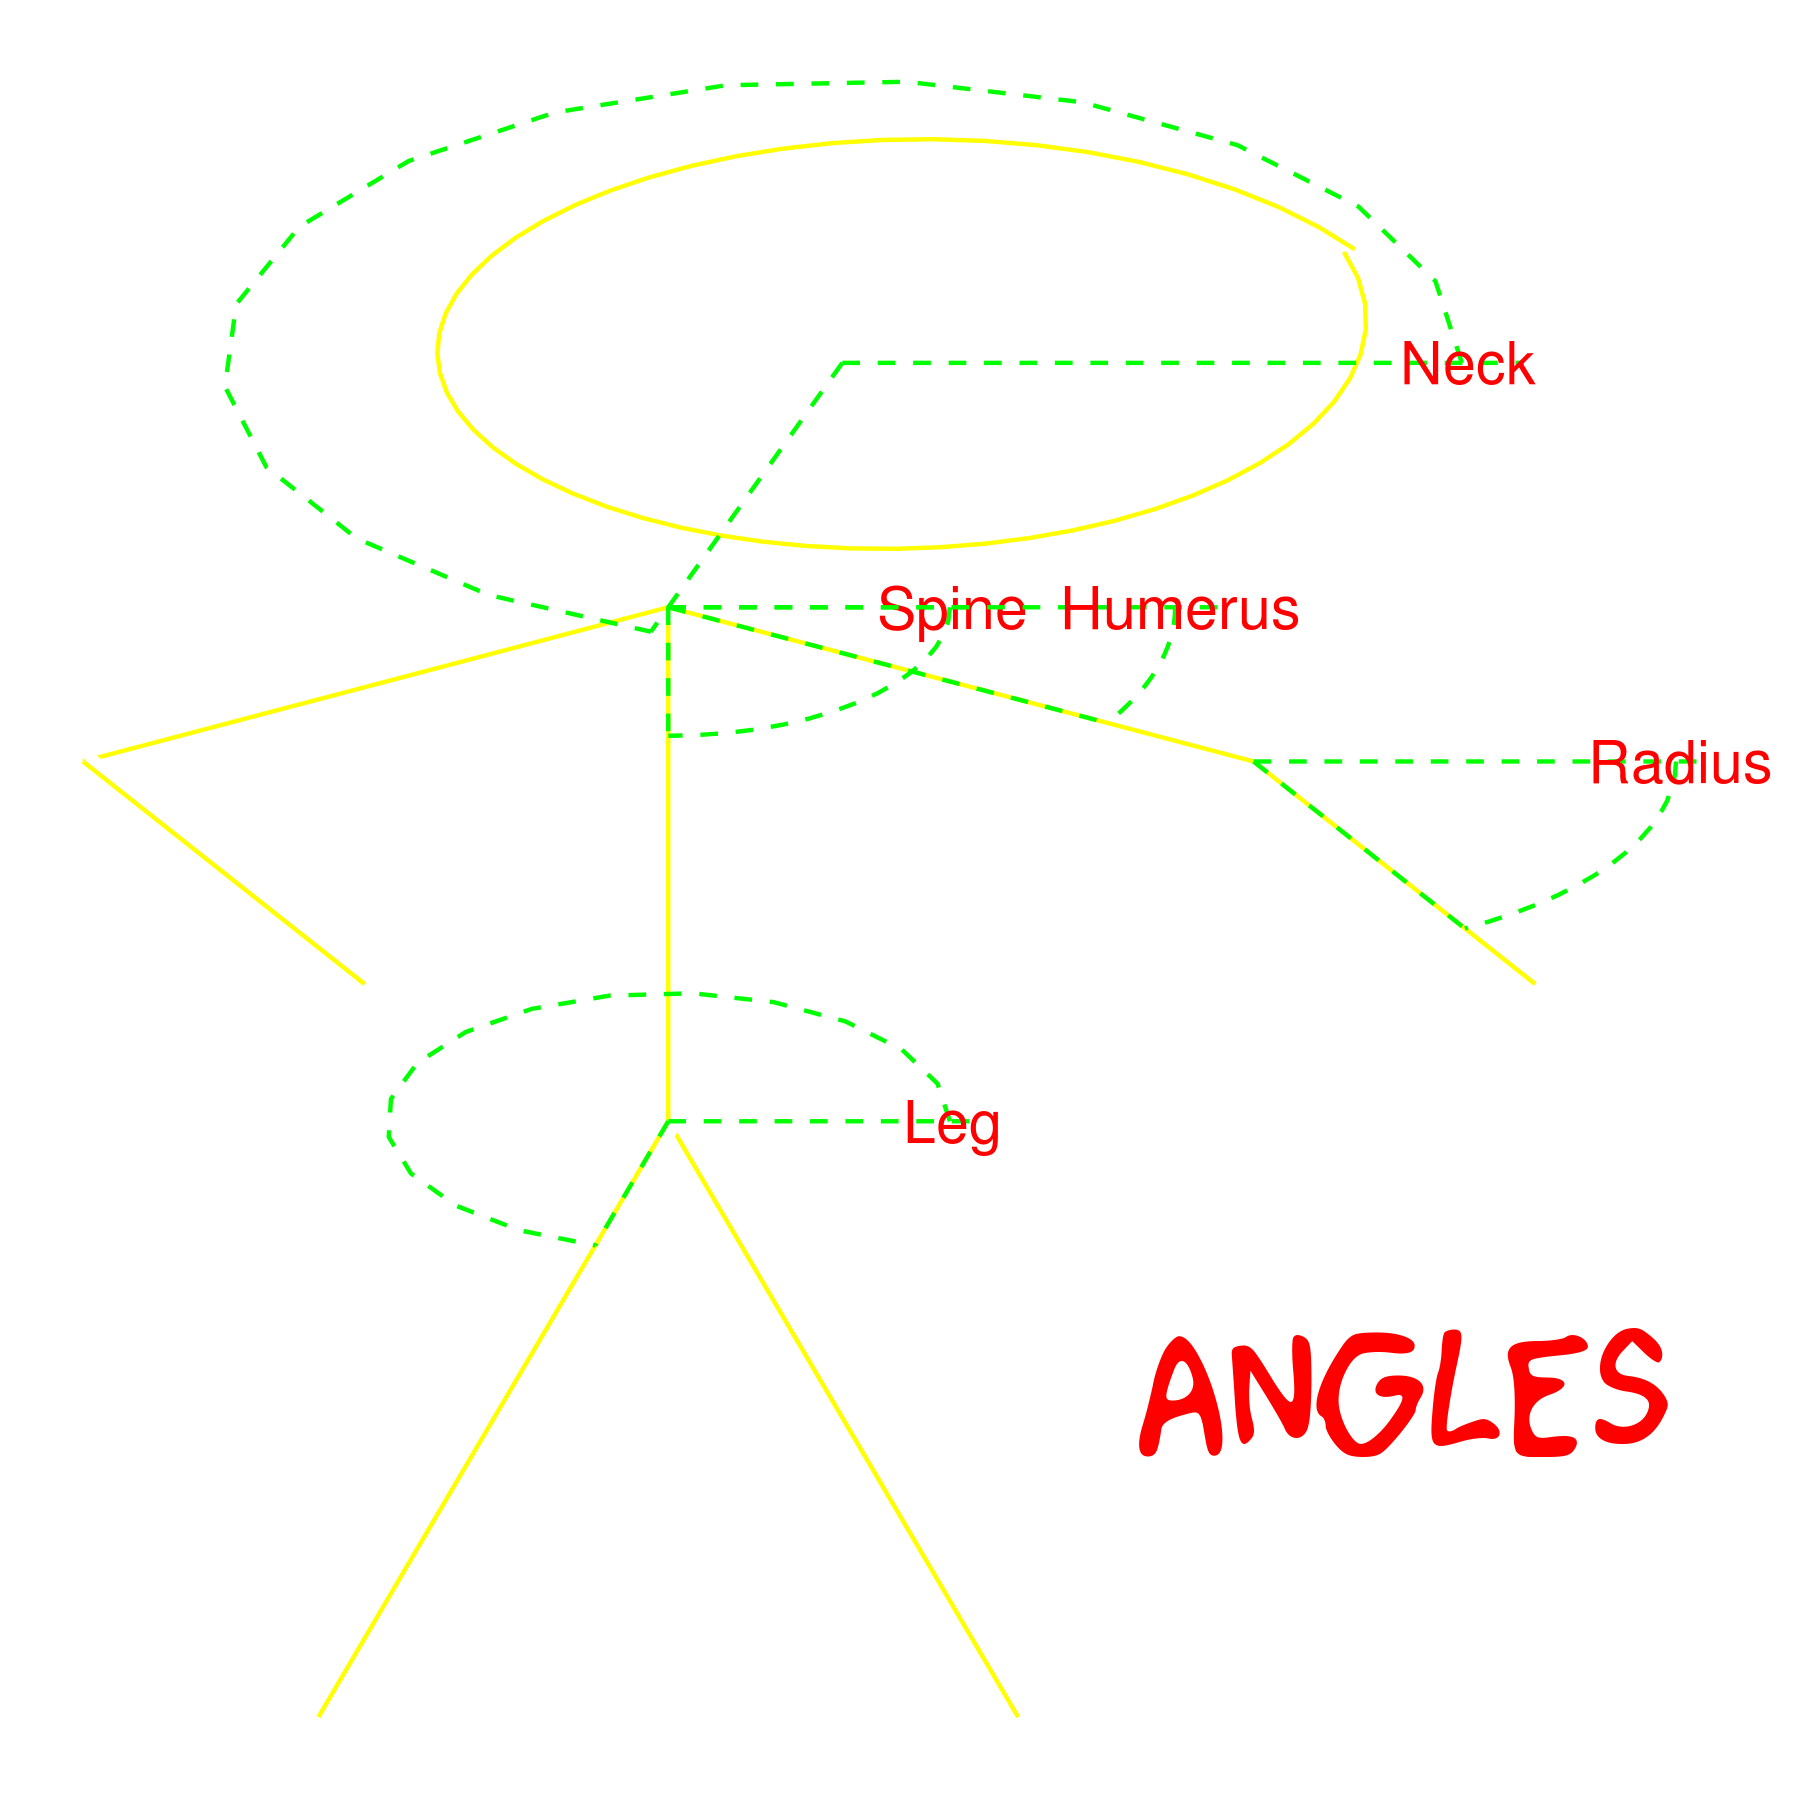
\includegraphics{xkcd-intro-angles}
\end{center}

\section{Mother's day}

\subsection{Bar chart}

\begin{center}
\begin{Schunk}
\begin{Sinput}
> mommy <- read.table(sep=" ",text ="
+ 8 100
+ 9 0
+ 10 0
+ 11 0
+ 12 0
+ 13 0
+ 14 100
+ 15 100
+ 16 500
+ 17 420
+ 18 75
+ 19 50
+ 20 100
+ 21 40
+ 22 0
+ ")
> names(mommy) <- c("hour","number")
> data <- mommy
> data$xmin <- data$hour - 0.25
> data$xmax <- data$xmin + 1
> data$ymin <- 0
> data$ymax <- data$number
> xrange <- range(8, 24)
> yrange <- range(min(data$ymin) + 10 , max(data$ymax) + 200)
> ratioxy <- diff(xrange)/diff(yrange)
> timelabel <-  function(text,x,y) {
+   if( "xkcd" %in% font.families()){
+     te1 <- annotate("text", x=x, y = y + 65, label=text, size = 6,family ="xkcd")
+   } else {
+     te1 <- annotate("text", x=x, y = y + 65, label=text, size = 6)}
+   list(te1,
+   xkcdline(aes(xbegin=xbegin, ybegin= ybegin, xend=xend,yend=yend),
+            data.frame(xbegin=x,ybegin= y + 50, xend=x,yend=y), xjitteramount = 0.5))
+   }
> n <- 1800
> set.seed(123)
> x <- runif(n, xrange[1],xrange[2] )
> y <- runif(n, yrange[1],yrange[2] )
> inside <- unlist(lapply(1:n, function(i) any(data$xmin <= x[i] & x[i] < data$xmax &
+                             data$ymin <= y[i] & y[i] < data$ymax)))
> x <- x[inside]
> y <- y[inside]
> nman <- length(x)
> sizer <- round(runif(nman, 1, 10),0)
> angler <- runif(nman, -10,10)
> if( "xkcd" %in% font.families()){
+ p <- ggplot() +
+   geom_text(aes(x,y,label="Mummy",angle=angler,hjust=0, vjust=0),
+             family="xkcd",size=sizer,alpha=0.3) +
+   xkcdaxis(xrange,yrange) +
+   annotate("text", x=16, y = 650,
+            label="Happy Mother's day", size = 16,family ="xkcd") +
+   xlab("daily schedule") +
+   ylab("Number of times mothers are called on by their children") +
+   timelabel("Wake up", 9, 125) + timelabel("School", 12.5, 90) +
+   timelabel("Lunch", 15, 130) +
+   timelabel("Homework", 18, 525) +
+   timelabel("Bath", 21, 110) +
+   timelabel("zzz", 23.5, 60)
+ } else {
+ p <- ggplot() +
+   geom_text(aes(x,y,label="Mummy",angle=angler,hjust=0, vjust=0),
+             size=sizer,alpha=0.3) +
+   xkcdaxis(xrange,yrange) +
+   annotate("text", x=16, y = 650,
+            label="Happy Mother's day", size = 16) +
+   xlab("daily schedule") +
+   ylab("Number of times mothers are called on by their children") +
+   timelabel("Wake up", 9, 125) + timelabel("School", 12.5, 90) +
+   timelabel("Lunch", 15, 130) +
+   timelabel("Homework", 18, 525) +
+   timelabel("Bath", 21, 110) +
+   timelabel("zzz", 23.5, 60)}
> p
\end{Sinput}
\end{Schunk}
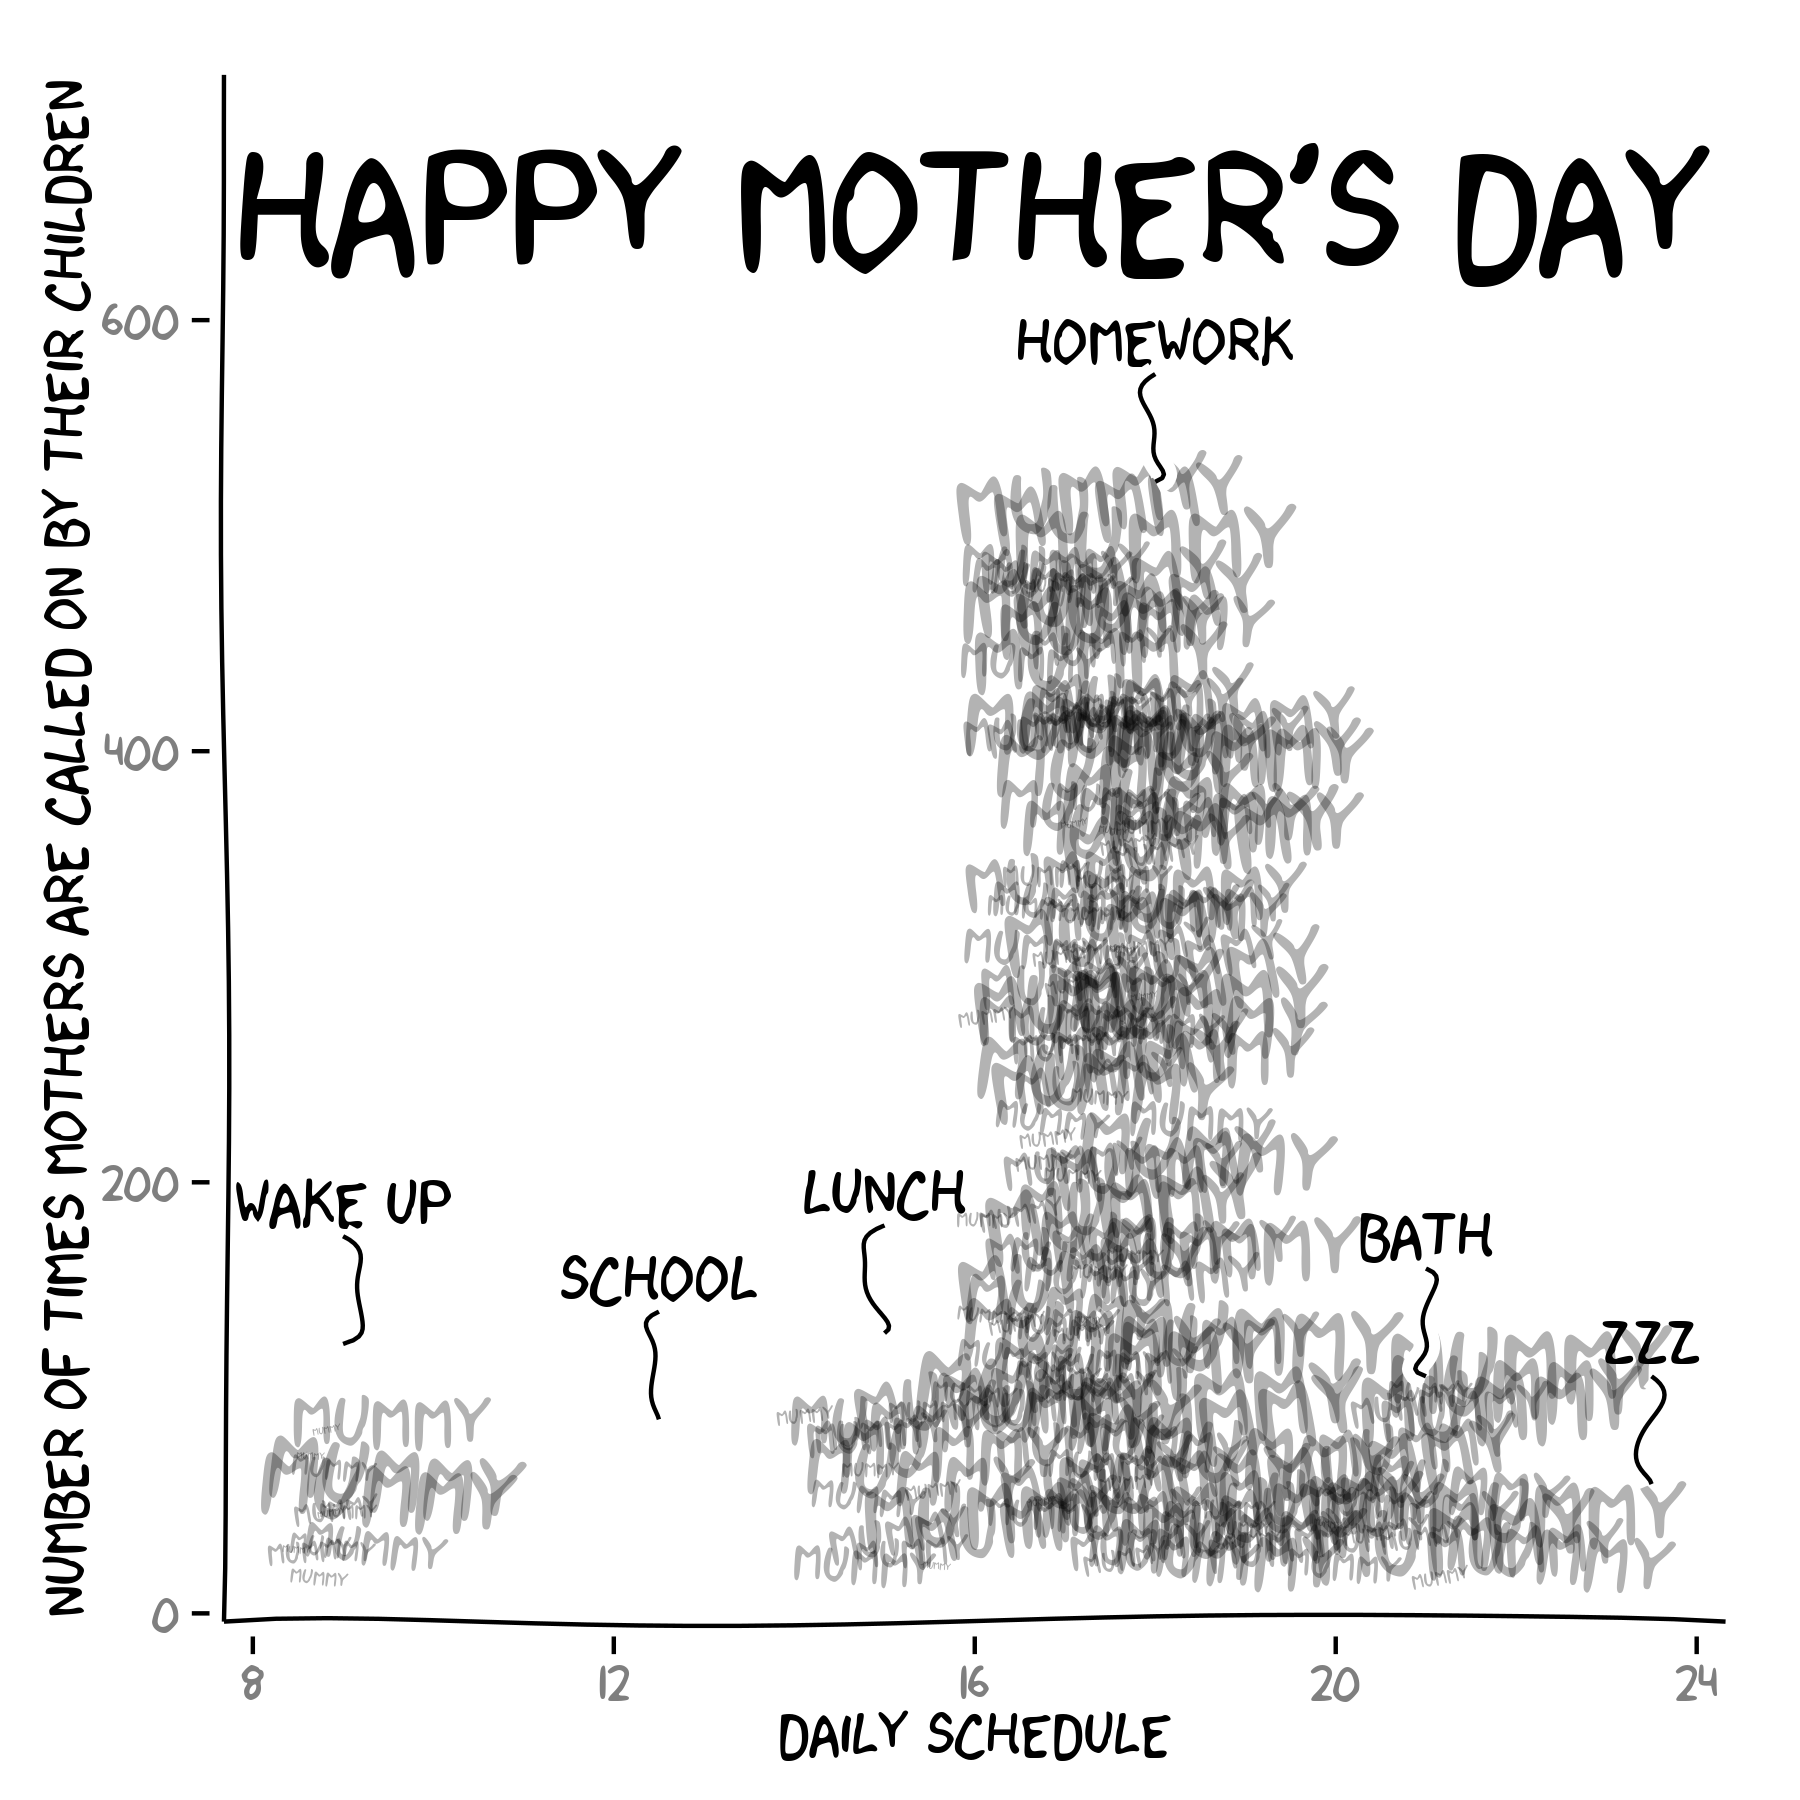
\includegraphics{xkcd-intro-motherday}

\end{center}
\section{Volunteers at C\'aritas Spain}

\subsection{Scatterplot}

\begin{center}
\begin{Schunk}
\begin{Sinput}
> volunteers <- data.frame(year=c(2007:2011), number=c(56470, 56998, 59686, 61783, 64251))
> xrange <- range(volunteers$year)
> yrange <- range(volunteers$number)
> ratioxy <-  diff(xrange) / diff(yrange)
> mapping <- aes(x,  y,
+                scale,
+                ratioxy,
+                angleofspine ,
+                anglerighthumerus,
+                anglelefthumerus,
+                anglerightradius,
+                angleleftradius,
+                anglerightleg,
+                angleleftleg,
+                angleofneck)
> dataman <- data.frame( x= c(2008,2010), y=c(63000, 58850),
+                       scale = 1000 ,
+                       ratioxy = ratioxy,
+                       angleofspine =  -pi/2  ,
+                       anglerighthumerus = c(-pi/6, -pi/6),
+                       anglelefthumerus = c(-pi/2 - pi/6, -pi/2 - pi/6),
+                       anglerightradius = c(pi/5, -pi/5),
+                       angleleftradius = c(pi/5, -pi/5),
+                       angleleftleg = 3*pi/2  + pi / 12 ,
+                       anglerightleg = 3*pi/2  - pi / 12,
+                       angleofneck = runif(1, 3*pi/2-pi/10, 3*pi/2+pi/10))
> datalines <- data.frame(xbegin=c(2008.3,2010.5),ybegin=c(63000,59600), 
+                         xend=c(2008.5,2010.3), yend=c(63400,59000))
> p <- ggplot() + geom_smooth(mapping=aes(x=year, y =number), data =volunteers,method="loess")
> if( "xkcd" %in% font.families()){
+ p + xkcdaxis(xrange,yrange) +
+   ylab("Volunteers at Caritas Spain") +
+   xkcdman(mapping, dataman) +
+   annotate("text", x=2008.7, y = 63700, label = "We Need\nVolunteers!", family="xkcd" ) +
+   annotate("text", x=2010.5, y = 60000, label = "Sure\nI can!", family="xkcd" ) +
+  xkcdline(aes(xbegin=xbegin,ybegin=ybegin,xend=xend,yend=yend),datalines, xjitteramount = 0.12) 
+ } else {
+ p + xkcdaxis(xrange,yrange) +
+   ylab("Volunteers at Caritas Spain") +
+   xkcdman(mapping, dataman) +
+   annotate("text", x=2008.7, y = 63700, label = "We Need\nVolunteers!") +
+   annotate("text", x=2010.5, y = 60000, label = "Sure\nI can!") +
+  xkcdline(aes(xbegin=xbegin,ybegin=ybegin,xend=xend,yend=yend),datalines, xjitteramount = 0.12) 
+ }
\end{Sinput}
\end{Schunk}
\includegraphics{xkcd-intro-016}
\end{center}

\subsection{Bar chart}

\begin{center}
    
\begin{Schunk}
\begin{Sinput}
> data <- volunteers
> data$xmin <- data$year - 0.1
> data$xmax <- data$year + 0.1
> data$ymin <- 50000
> data$ymax <- data$number
> xrange <- range(min(data$xmin)-0.1, max(data$xmax) + 0.1)
> yrange <- range(min(data$ymin)+500, max(data$ymax) + 1000)
> mapping <- aes(xmin=xmin,ymin=ymin,xmax=xmax,ymax=ymax)
> p <- ggplot() + xkcdrect(mapping,data) + 
+   xkcdaxis(xrange,yrange) +
+   xlab("Year") + ylab("Volunteers at Caritas Spain")
> p
\end{Sinput}
\end{Schunk}
\includegraphics{xkcd-intro-017}

\subsection{Bar chart}

\begin{Schunk}
\begin{Sinput}
> data <- volunteers
> data$xmin <- data$year - 0.1
> data$xmax <- data$year + 0.1
> data$ymin <- 50000
> data$ymax <- data$number
> xrange <- range(min(data$xmin) - 0.1, max(data$xmax) + 0.1)
> yrange <- range(min(data$ymin) +500 , max(data$ymax) + 1000)
> ratioxy <- diff(xrange)/diff(yrange)
> plotmen <- function(x,y, scale,ratioxy,...){
+  mapping <- aes(x,  y,
+                  scale,
+                  ratioxy,
+                  angleofspine ,
+                  anglerighthumerus,
+                  anglelefthumerus,
+                  anglerightradius,
+                  angleleftradius,
+                  anglerightleg,
+                  angleleftleg,
+                  angleofneck)
+   n <- length(x)
+   data <- data.frame(x=x,
+                      y=y,
+                      scale = scale,
+                      ratioxy = ratioxy,
+                      angleofspine = runif(n, - pi/2 - pi/3, -pi/2 + pi/3),
+                      anglerighthumerus = runif(n, -pi/6- pi/10, - pi/6 + pi/10),
+                      anglelefthumerus = runif(n, pi + pi/6 -pi/10, pi + pi/6 + pi/10),
+                      anglerightradius =  runif(n, -pi/4, pi/4),
+                      angleleftradius =  runif(n, pi -pi/4, pi + pi/4),
+                      anglerightleg = runif(n,  3* pi/2 + pi/12 , 3* pi/2  + pi/12 + pi/10),
+                      angleleftleg = runif(n, 3* pi/2  - pi/12 - pi/10, 3* pi/2 - pi/12 ),
+                      angleofneck = runif(n, -pi/2-pi/10, -pi/2 + pi/10))
+   xkcdman(mapping,data,...)
+ }
> volun <- c("Miguel","Jose","Rocio","Maria","Emilio",
+            "Pilar","Tata","Violeta","Titi","Alex","Dani")
> positionx <- seq(2007,2011, length.out=length(volun))
> set.seed(123)
> positionx <- positionx[sample(1:length(volun),length(volun))]
> positiony <- seq(54000,65000,length.out = length(volun))
> a <- ggplot() + 
+   xkcdrect(mapping,data,fill="yellow",colour="red") + 
+   xkcdaxis(xrange,yrange) +
+   xlab("Year") + ylab("Volunteers at Caritas Spain")
> b <- a + plotmen(positionx, positiony,1000, ratioxy) 
> if( "xkcd" %in% font.families()){
+ c <- b + annotate("text", 
+                   x= positionx, y= positiony, 
+                   label=volun, family="xkcd",size=3) 
+ } else {
+ c <- b + annotate("text", 
+                   x= positionx, y= positiony, 
+                   label=volun,size=3) 
+ }
> c
\end{Sinput}
\end{Schunk}
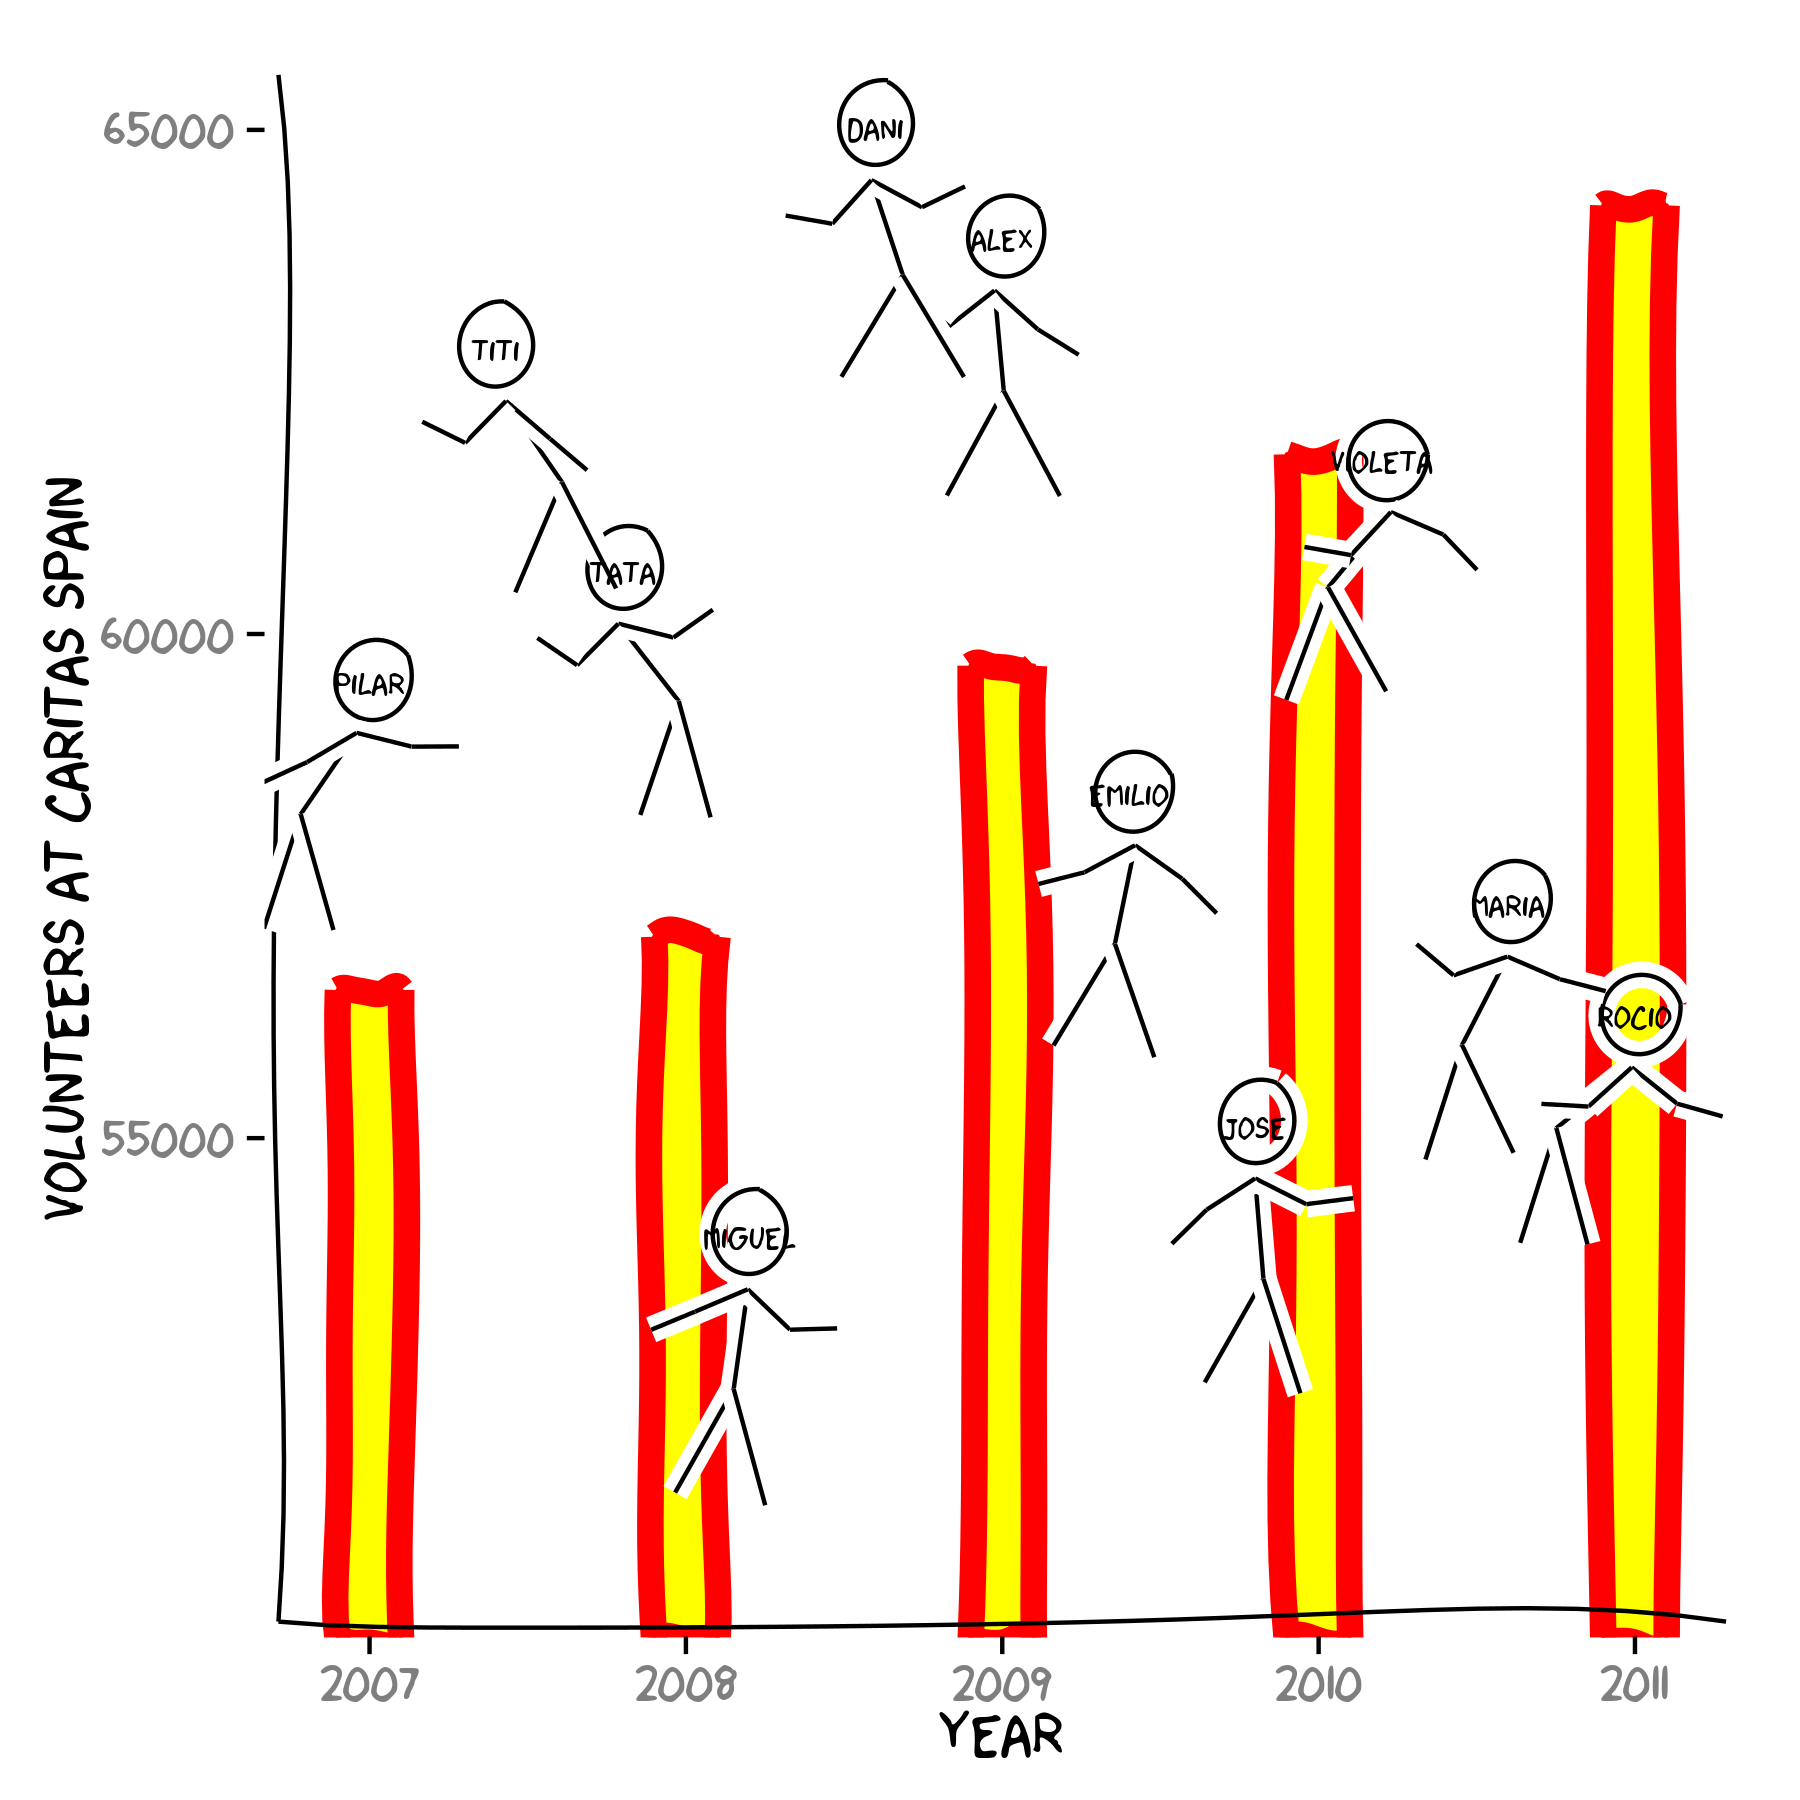
\includegraphics{xkcd-intro-CaritasSpain}
\end{center}



\section{References}


    Hadley Wickham 2012. ggplot2 \url{http://ggplot2.org/}
    
    Randall Munroe. A webcomic of romance, sarcasm, math, and language
    \url{http://xkcd.com/}

    Various Authors 2012. How can we make xkcd style graphs in R? \url{http://stackoverflow.com/questions/12675147/how-can-we-make-xkcd-style-graphs-in-r}

    % fibosworld 2013. Change fonts in ggplot2, and create xkcd style graphs \url{http://fibosworld.wordpress.com/2013/02/17/change-fonts-in-ggplot2-and-create-xkcd-style-graphs/}

    Yixuan Qiu, 2014, sysfonts, \url{http://cran.r-project.org/web/packages/sysfonts/index.html}
    
    Yixuan Qiu, 2014, showtext, \url{http://cran.r-project.org/web/packages/showtext/index.html}
    
\end{document}


